\documentclass{ximera}

\input{../../preamble.tex}

\author{Bobby Ramsey}

\begin{document}
\begin{exercise}

	Suppose $\theta$ is a central angle of a circle with radius $r$, as shown below.
	\begin{center}
	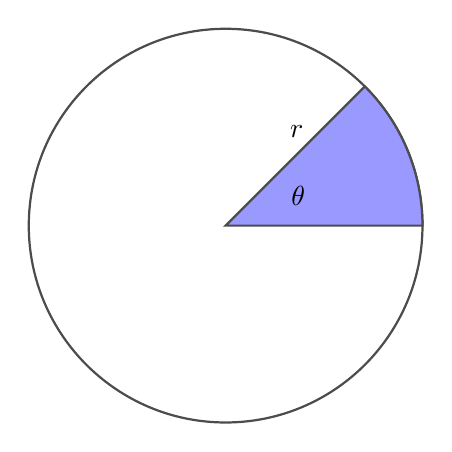
\begin{tikzpicture}[draw=black!70,thick]
		\draw circle (2.5cm);
		\filldraw[fill=blue!40] 
			(45:2.5cm) %node[right] {Q}
			-- (0,0) %node[left below] {$\theta$}
			-- (0:2.5cm) %node[left] {P} 
		arc[start angle=0, end angle=45, radius=2.5cm]
			-- cycle;
		\node at (53:1.5cm) {$r$};
		\node at (22.5:1cm) {$\theta$};
	\end{tikzpicture}
	\end{center}	
	
	What is the area and circumference of the circle?
	\begin{align*}
		\text{ Area } &= \answer{\pi r^2}\\ \\
		\text{ Circumference } &= \answer{ 2 \pi r}
	\end{align*}

	\begin{exercise}
		What proportion of the circle lies within the sector 
		subtended by $\theta$?  $\answer{ \frac{\theta}{2\pi}}$.
		\begin{hint}
			What is the central angle inside the sector?\\
			What is the angle determined by an entire rotation?
		\end{hint}
		\begin{exercise}
			What is the area and arclength of the circle subtended by the angle $\theta$?
			
			\begin{align*}
				\text{ Area } &= \answer{\frac{r^2 \theta}{2}}\\ \\
				\text{ Arc length } &= \answer{ r \theta}
			\end{align*}
			\begin{hint}
				Total amount * proportion
			\end{hint}
			\begin{exercise}
				If $\theta$ is a central angle in a unit circle which 		
				subtends a sector with area 2, find the arc length determined
				by that sector.
				
				\[ \text{Arc length } = \answer{4} \]
			\end{exercise}
		\end{exercise}
	\end{exercise}


\end{exercise}
\end{document}